% !TEX root = ../TSG_Administrator's_Guide_Latest_EN.tex
%
\pdfbookmark[0]{Policies}{Policies}
\chapter*{\hypertarget{link:Policies}{Policies}}
\label{sec:policies}

The policy is the axis around which most features of TSG revolve. Many TSG settings end up relating to or being associated with the policies and the traffic they govern. 
Any traffic going through TSG has to be associated with a policy. These policies are essentially discrete compartmentalized sets of instructions that control the traffic 
flow going through TSG. These instructions control where the traffic goes, how it is processed, if it is processed, and whether or not it is allowed to pass through the gate.


When TSG receives a connection packet, it analyzes the source, destination, application and corresponding filters. Using this information, 
TSG attempts to locate a security policy that matches the packet. If a policy matches the parameters, then TSG takes the required action for that policy. 
If it is Allow, the traffic is allowed to proceed to the next step. If the action is Deny, the traffic is not allowed to proceed. If the action is Monitor, 
the traffic is scanned and a log is generated. If it is Intercept, the traffic is intercepted and relative proxy policy will be applied. 

{
\color{linkblue}
\hyperlink{link:Policy Concepts}{> Policy Concepts} \\
\hyperlink{link:Security Policy}{> Security Policy} \\
\hyperlink{link:Proxy Policy}{> Proxy Policy}\\
\hyperlink{link:Schedules}{> Schedules}\\
\hyperlink{link:Verify Policy Rules}{> Verify Policy Rules}\\
}
\clearpage

\pdfbookmark[1]{Policy Concepts}{Policy Concepts}
\section*{\hypertarget{link:Policy Concepts}{Policy Concepts}}
\label{sec:policies:concepts}

Policies allow you to enforce rules and take action. From TSG’s perspective, network packets are first resembled to a session, and identified as many manageable attributes. 
For example, a TLS session could be parsed to attributes as IP address, SNI, certificate and so on. For effective management, user could define policy rules with TSG user interface. 


A policy rule combines with several conditions and one action. The action determines how to control the traffic, and action parameters are managed in policy profiles. 
Profiles are elaborated in chapter \hyperlink{link:Certificate Managements}{\color{linkblue}{Certificate Managements}}  and chapter \hyperlink{link:Proxy Profiles}{\color{linkblue}{Proxy Profiles}}. 
The conditions describe attributes of applicable traffic, and they are organized by policy objects. 
While policy objects enable you to identify traffic to enforce policies, policy profiles help you define further action.  Traffic must match all conditions of a policy before taking its action. 
Traffic matching one item of an object means it satisfies the object. In short, objects in one policy are “AND” relation, items and subordinate object in one object are “OR” relation. 


You can identify a policy rule by its name or ID number. The policy ID for a rule never changes even if you modify the rule, such as when you change the rule name. 
The policy ID allows you to track the rule across rules even after you disable the rule.


\notemark\textit{Note that activation of policy rules on all devices is no more than 1 minute. 
For details about capacities of policies and URLs/URIs, and other system parameters, see \textcolor{darkblue}{\textbf{\underline{ADC-L404 Datasheet}}}.}

\pdfbookmark[2]{Rule Types}{Rule Types}
\subsection*{\hypertarget{link:Rule Types}{Rule Types}}
\label{sec:policies:concepts:types}

TSG supports a variety of policy types that work together to safely enable applications on your network. The different types of policy rules that you can create on TSG are:\\
%\begin{table}[h]
\begin{longtable}{p{0.17\textwidth}|p{0.77\textwidth}}   
%    \begin{tabularx}{\textwidth}{p{0.17\textwidth}|p{0.77\textwidth}} 
    \rowcolor{black}\multicolumn{1}{l!{\color{white}\vrule width 0.5pt}}{\textcolor{white}{Policy Type}}  & \textcolor{white}{Description} \\\hline                                                                                                                                                          
    Security & Determine whether to allow, deny, monitor or intercept a session based on traffic attributes such as the IP addresses, subscriber ID, APP ID and protocol fields. 
    For more details, see \hyperlink{link:Security Policy}{\color{linkblue}{Security Policy}}.\\\hline                                                                                                          
    \begin{tabular}{l}\tabincell{l}{Proxy\\ Manipulation}\end{tabular} & Instruct the proxy how to manipulate (including allow, deny, monitor, redirect, replace, hijack and insert), 
    a session based on traffic attributes such as the source and destination IP address, the subscriber ID, and filter, including host, URL, 
    request header, response header, request content and response content. Encrypted traffic Identified will be decrypted for further control. 
    Manipulation requires targeted sessions are intercepted in security policies. For more details, see \hyperlink{link:Proxy Policy}{\color{linkblue}{Proxy Policy}}.\\\hline 
%    \end{tabularx}
\end{longtable} 
%end{table}

\pdfbookmark[2]{Policy Conditions}{Policy Conditions}
\subsection*{\hypertarget{link:Policy Conditions}{Policy Conditions}}
\label{sec:policies:concepts:conditions}

Each rule has a set of conditions. All criteria need to match if the rule action is to be used. The order of each condition in the list is irrelevant. 
A condition consists of an object type from the list of object types used for traffic identification, an operator (only support equals for now) and a specific object of that type. 
If a connection matches all the objects set to "equals" in the rule, the rule will apply to the connection.


Policy objects server as policy conditions. There are four types of conditions at most in each policy, namely: Source, Destination, Application and corresponding Filter. 
You can view which objects are referenced as conditions by selecting \textbf{Policies} > \textbf{Security} or \textbf{Policies} > \textbf{Proxy}, then double click the policy in the list.


A policy object consists of collective items that groups discrete identities such as IP addresses, URLs, applications, or user accounts. 
You can define an object with a set of items or a set of subordinate objects and reuse it in multiple policies. 


\notemark\textit{Consider a Source, Destination, Application and each member of a Filter as a condition. A policy contains 8 conditions at most. 
The relation between each condition is “and”. The relation within each condition is “or”. 
Take HTTP as an example, possible values of its Filter can be Host, URL, Request Header etc. If you add two Hosts for Filter, the relation between each Host is also “and”.}


For more details about policy objects, see \hyperlink{link:Objects}{\color{linkblue}{Objects}}.


\pdfbookmark[2]{Policy Hierarchy and Evaluation Order}{Policy Hierarchy and Evaluation Order}
\subsection*{\hypertarget{link:Policy Hierarchy and Evaluation Order}{Policy Hierarchy and Evaluation Order}}
\label{sec:policies:concepts:order}

TSG firewall uses a network stack to process the packet, like the OSI model. When a network packet passes through, it will be parsed and resembled to a network session. 
And the reassembled network session is decoded to identify the embedded content. At each step of the decoding process, all applicable fields of the application protocol, 
the application, and the file are extracted and stored. These extracted attributes provide context to the content that was extracted from the data. 
This extracted attributes and content provide comprehensive visibility into network traffic. With this deep visibility, 
security policies can be fine grained crafted to detect and manage network threats.


Based aforementioned design, security policy rules are enforced as following \textbf{inspection layers}:
\begin{description}[leftmargin=0pt,itemindent=0em,itemsep=0.5ex]
    \item
    \begin{enumerate}
        \item 	Packet layer: The firewall parses IP fragments, reassembles using the defragmentation process, and then parses IP header and TCP/UDP protocol headers if applicable. As application identification is on all layers, the identified application as well as IP address, ASN and Subscriber ID is used as key to find rule match. Because the application is not necessarily known in the first packets, it can take several packets to determine what the underlying application is, and rules without specifying application will be enforced in advance.
        \item 	Session layer: Packets are reassembled to network session and decoded to traffic attributes, e.g. TLS SNI (TLS handshake option), HTTP Host, Mail addresses and DNS QNAME.
        \item 	Content layer: Content that extracted from one session or more sessions are applicable for keywords scan, e.g. HTTP request body and Mail attachment.
    \end{enumerate}
 \end{description}
Within the layer, traffic attributes are not acquired simultaneously, which is known as \textbf{parsing stages}. This design offers stateful security functions at the application layer, 
and the effectiveness of policy enforcement. The parsing stages of common protocols are listed in table below.\\
%\begin{table}[h]
\begin{longtable}{p{0.17\textwidth}|p{0.77\textwidth}}   
    %\begin{tabularx}{\textwidth}{p{0.17\textwidth}|p{0.77\textwidth}}
    \rowcolor{black}\multicolumn{1}{l!{\color{white}\vrule width 0.5pt}}{\textcolor{white}{Protocols}}  & \textcolor{white}{Attributes Parsing Stages} \\\hline                                                                                                                                                          
    HTTP &  \begin{tabular}{l}
            1.	Host, URL \\
            2.	Request Header \\
            3.	Request Body \\
            4.	Response Header \\
            5.	Response Body 
            \end{tabular}\\ \hline                                                                                                            
    TLS/SSL &   \begin{tabular}{l}  
                1.	SNI \\
                2.	CN, SAN 
                \end{tabular}\\ \hline                                                                                                          
    DNS & QNAME\\\hline 
    MAIL &  \begin{tabular}{l}
            1.	Account\\
            2.	From, To, Subject\\
            3.	Content\\
            4.	Attachment File Name\\
            5.	Attachment File 
            \end{tabular}\\\hline 
    FTP &   \begin{tabular}{l}
            1.	Account\\
            2.	URI\\
            3.	Content 
            \end{tabular}\\\hline 
    %\end{tabularx}
%\end{table}
\end{longtable}
As the firewall receives more packets and do more in-depth inspection, more traffic attributes and content are ready for policy enforcement, which is shown in figure below.\\


%\begin{figure}[htb]
	%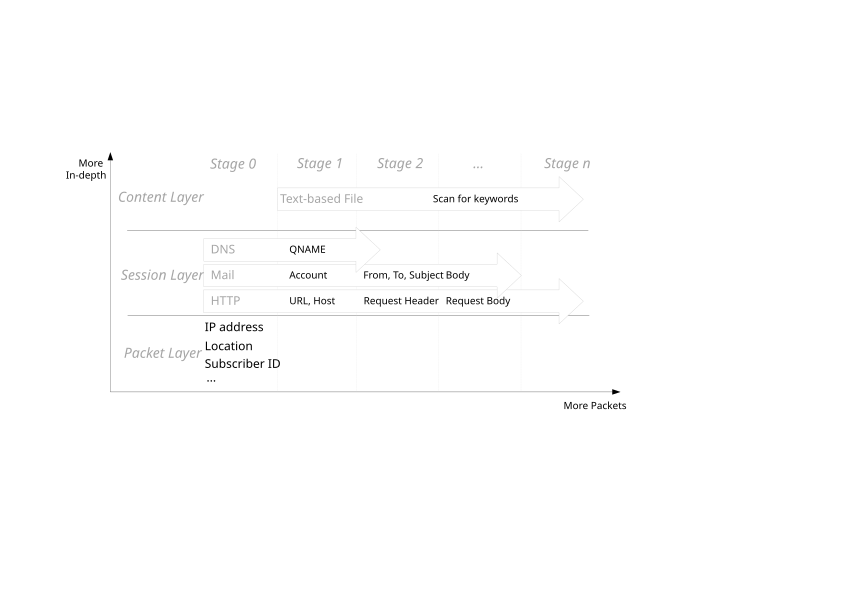
\includegraphics[width=\textwidth]{images/policy_enforcement_stage_v2.svg}
	%\caption{Figure: Inspection Stage}
	%\label{fig:system:policy_enforcement_stage_v2}
%\end{figure}

%\begin{figure}
%    \centering
%    \def\svgwidth{\columnwidth}
%    \input{../images/policy_enforcement_stage_v2.pdf_tex}
%\end{figure}

\begin{figure}[htb]
    \centering
    \includesvg{\columnwidth}{../images/policy_enforcement_stage_v2}
    %\caption{Figure}
\end{figure}


It is highly likely that even after only a relatively small number of policies have been created that there will be some that overlap 
or are subsets of the parameters that the policies use to determine which policy should be matched against the incoming traffic. 
When this happens there has to be a method to determine which policy should be applied to the packet. The method which is used by TSG is the policy hierarchy. 
In another words, policies with lower inspection layers and earlier parsing stages are precedent. For example, a HTTP session, its URL appears before response body. 
That’s why policy rules that inspect HTTP response body, are always evaluated after ones that inspect URL.


\notemark\textit{A policy rule that combines with condition fields of different layers and stages are evaluated at the last layer and stage. 
Rule stage is decided by policy condition fields; and rule modification may change the rule stages.}


As firewall maybe unable to determine the exact application from the first packet, a session may be allowed through the firewall as undecided 
until the application is identified, at which time the security rules are re-evaluated and an appropriate action is taken.


For more details about how TSG process packet flow, please see \hyperlink{link:Appendix E TSG Packet Flow}{\color{linkblue}{Appendix E TSG Packet Flow}}.

\pdfbookmark[1]{Security Policy}{Security Policy}
\section*{\hypertarget{link:Security Policy}{Security Policy}}
\label{sec:policies:security}

Security policies determine whether to deny, allow, monitor or intercept a session based on initial session attributes, 
such as the subscriber ID, IP addresses, ports, protocols and applicable protocol fields (e.g. TLS SNI). 
On TSG, security policy rules are enforced by firewall module.


All traffic passing through the firewall is matched against a session and each session is matched against a security policy rule. 
When a session match occurs, the firewall applies the matching security policy rule to bidirectional traffic in that session (client to server and server to client). 
For traffic that doesn’t match any defined rules, the default rule applies. The default rule is predefined to allow all traffic for firewall policy check. 
Although the default rule is read-only by default, you can override them and change a limited number of settings, including the tags, action (allow or deny) and log settings.


A packet is matched against the first rule that meets the defined criteria and, after a match is triggered, subsequent rules are not evaluated. 
Session that matches a rule generates a log entry at the end of the session in the security event log if you enable logging for that rule. 
The logging options are configurable for each rule.

\pdfbookmark[2]{Components of a Security Policy Rule}{Components of a Security Policy Rule}
\subsection*{\hypertarget{link:Components of a Security Policy Rule}{Components of a Security Policy Rule}}
\label{sec:policies:security:component}

The Security policy rule construct permits a combination of the required and optional fields as detailed in the following table:\\


\begin{longtable}{p{0.15\textwidth}|p{0.23\textwidth}|p{0.54\textwidth}}   
    \rowcolor{black}\multicolumn{1}{l!{\color{white}\vrule width 0.5pt}}{\textcolor{white}{\begin{tabular}{l}Required/\\Optional\end{tabular}}}  & \multicolumn{1}{l!{\color{white}\vrule width 0.5pt}}{\textcolor{white}{Field}} & \textcolor{white}{Description}\\\hline                                                                                                                                                          
    \multirow{3}{*}{Required} & Name & A label (up to 128 characters) that identifies the rule.\\ \cline{2-3}
                              & Action & Specifies an Allow, Deny, Monitor or Intercept action for the traffic based on the criteria you define in the rule. For more details, see \hyperlink{link:Security Actions}{\color{linkblue}{Security Policy Actions}}. \\ \cline{2-3}
                              & Application & The application that you wish to control. It provides application control and visibility in creating security policies that block unknown applications, while enabling, inspecting, and shaping those that are allowed. For more information, see \textbf{Objects} > \textbf{Applications} and \hyperlink{link:Appendix B Predefined Applications}{\color{linkblue}{Appendix B Predefined Application}}.\\ \hline                                                                                                        
    \multirow{9}{*}{Optional} & Source & Define host IP addresses, address groups, Subscriber ID, IP Learning, or Geographic enforcement.\\ \cline{2-3}
                              & Destination & The location or destination for the packet. Define host IP addresses, address groups, IP Learning, or Geographic enforcement.\\ \cline{2-3}
                              & Filter & All web traffics are compared against the filtering, giving you a way to safely control how your users interact with online content. You will have Filter available when you select only one of the following protocols: HTTP, SSL, DNS, MAIL, FTP and QUIC in Applicationfield.\\ \cline{2-3}
                              & Tag & A keyword or phrase that help you to identify the policy. \\ \cline{2-3}
                              & Effective Devices & Select the devices that the security rule will be applied.\\ \cline{2-3}
                              & Schedule & Schedule when (day and time) the security rule should be in effect. \\ \cline{2-3}
                              & Log Session & When enabled, traffic that match security policies will be logged in Security Event Logs. \\ \cline{2-3}
                              & Description & A text field, up to 1024 characters, used to describe the rule. \\ \cline{2-3}
                              & Enabled & Only enabled policies will be enforced.\\ \hline                                                                                                 
\end{longtable}

\pdfbookmark[2]{Actions}{Security Actions}
\subsection*{\hypertarget{link:Security Actions}{Actions}}
\label{sec:policies:security:action}

For traffic that matches the attributes defined in a security policy, you can apply the following actions:\\


\begin{longtable}{p{0.12\textwidth}|p{0.82\textwidth}}   
    \rowcolor{black}\multicolumn{1}{l!{\color{white}\vrule width 0.5pt}}{\textcolor{white}{Action}}  & \textcolor{white}{Description} \\\hline                                                                                                                                                          
    Allow &  The traffic is allowed to proceed to the next step.\\ \hline                                                                                                            
    Deny &  \begin{tabular}{l}  
            The traffic is not allowed to proceed. There are 5 Sub Action to \\
            select, they are Drop, RST (TCP reset attack), Block, Alert and \\
            Redirect.\\
            Sub Action of Deny:\\
            \textbf{Drop}, silently drops the traffic.\\
            \textbf{RST}, sends a TCP reset to the client-side device.\\
            \textbf{Block}, sends 403/404 return code and customized content to \\
            the client.\\
            \textbf{Alert}, sends 200/204 return code and customized content to the \\
            client.\\
            \textbf{Redirect}, redirects to the link set in the policy configuration.
            \end{tabular}\\ \hline                                                                                                          
    Intercept & Intercept HTTP/HTTPS traffic for proxy. If the traffic use SSL/TLS, it will be decrypted.\\\hline 
    Monitor &  Scan all allowed traffic and generate a detailed log.\\\hline 
\end{longtable}

\pdfbookmark[2]{Applications and Filters}{Security Applications and Filters}
\subsection*{\hypertarget{link:Security Applications and Filters}{Applications and Filters}}
\label{sec:policies:security:filter}

AppSketch is a traffic classification system available in TSG firewalls, determines what an application is irrespective of port, protocol, 
encryption or any other evasive tactic used by the application. It applies multiple classification mechanisms, (including application signatures, 
application protocol decoding, heuristics, and machine learning) to your network traffic stream to accurately identify applications.


Applications enables visibility into the applications on the network, so you can learn how they work and understand their behavioral characteristics 
and their relative risk. When you define policy rules to control traffic, applications begin to classify traffic without any additional configuration.


\begin{longtable}{p{0.14\textwidth}|p{0.19\textwidth}|p{0.58\textwidth}}   
    \rowcolor{black}\multicolumn{2}{l!{\color{white}\vrule width 0.5pt}}{\textcolor{white}{Applications Type}}  & \textcolor{white}{Description}\\\hline                                                                                                                                                          
    \multirow{3}{*}{Application} & Basic Protocols & Network protocols ensure that computer network devices can transmit and receive data using a common language regardless of their different designs, hardware or infrastructures. 
    List all 50 basic protocols: 
    
    
    Unknown\_TCP, Unknown\_UDP, Unknown\_Other, DNS, FTP, FTPS, HTTP, HTTPS, ICMP, IKE, IMAP, MAIL, IMAPS, IPSEC, XMPP, L2TP, NTP, POP3, POP3S, PPTP, QUIC, SIP, SMB, SMTP, SMTPS, SPDY, SSH, SSL, SOCKS, TELNET, DHCP, RADIUS, OPENVPN, STUN, TEREDO, DTLS, DoH, ISAKMP, MDNS, NETBIOS, NETFLOW, RDP, RTCP, RTP, SLP, SNMP, SSDP, TFTP, BJNP, LDAP, RTMP, RTSP. 
    \\ \cline{2-3}
                                 & \tabincell{l}{Predefined\\ Applications} & TSG has various predefined applications. \\ \cline{2-3}
                                 & \tabincell{l}{Customized\\ Applications} & TSG allows you create custom applications and reference the customized application objects in policy.\\\hline
    Selector & Selector & TSG allows you dynamically group applications based on application properties that you define into one object Selector. It is available for Action Allow and Deny. For more details, see \hyperlink{link:Application Selector}{\color{linkblue}{Application Selector}}.    \\ \hline 
    Group & Group & An application group is an object that contains applications that you want to treat similarly in a policy. It is available for Action Allow and Deny. For more details, see \hyperlink{link:Application Group}{\color{linkblue}{Application Group}}.    \\ \hline                                                                                                 
\end{longtable}


You will have Filter available when you select only one of the following protocols: HTTP, SSL, DNS, MAIL, FTP and QUIC. 
The following table lists different Filter fields for each protocol and the available object type you can select for each filter field, 
it also shows whether each filter field support allow, deny, monitor and intercept action or not. 


%
    %\rowcolor{black}\multirow{2}{*}{\multicolumn{1}{@{}l!{\color{white}\vrule width 0.5pt}}{\textcolor{white}{Protocol}}}  & \multirow{2}{*}{\multicolumn{1}{@{}l!{\color{white}\vrule width 0.5pt}}{\textcolor{white}{Filter Field}}} & 
    %\multirow{2}{*}{\multicolumn{1}{@{}l!{\color{white}\vrule width 0.5pt}}{\textcolor{white}{Available Object}}} & \multicolumn{4}{@{}l}{\textcolor{white}{Applicable Actions}} 
    %&\textcolor{white}{Applicable Actions} &\textcolor{white}{Applicable Actions} &\textcolor{white}{Applicable Actions}
    %\multicolumn{1 !{\color{white}\vrule width 0.5pt}}{\textcolor{white}{Protocol}}   
    %\textcolor{white}{Protocol}
    %!{\color{white}\vrule width 0.5pt}
%\begin{longtable}{p{0.16\textwidth}|p{0.17\textwidth}|p{0.18\textwidth}|p{0.1\textwidth}|p{0.1\textwidth}|p{0.11\textwidth}|p{0.12\textwidth}}
    %\setlength{\arrayrulewidth}{2pt}
\begin{longtable}{p{0.13\textwidth}|p{0.15\textwidth}|p{0.14\textwidth}|p{0.07\textwidth}|p{0.07\textwidth}|p{0.11\textwidth}|p{0.11\textwidth}} 
    \rowcolor{black}
    \multicolumn{1}{l !{\vlinewhite}}{} &
    \multicolumn{1}{l !{\vlinewhite}}{}  & 
    \multicolumn{1}{l !{\vlinewhite}}{} & 
    \multicolumn{4}{c}{\textcolor{white}{Applicable Actions}} \\ 
    \arrayrulecolor{white}\cline{4-7}  
    \rowcolor{black}
    \multicolumn{1}{l !{\vlinewhite}}{\multirow{-2}{*}{\textcolor{white}{Protocol}}} & 
    \multicolumn{1}{l !{\vlinewhite}}{\multirow{-2}{*}{\textcolor{white}{Filter Field}}} &
    \multicolumn{1}{l !{\vlinewhite}}{\multirow{-2}{*}{\textcolor{white}{\tabincell{l}{Available\\ Object}}}} & 
    \multicolumn{1}{l!{\color{white}\vrule width 0.5pt}}{\textcolor{white}{Allow}}  & 
    \multicolumn{1}{l!{\color{white}\vrule width 0.5pt}}{\textcolor{white}{Deny}}  & 
    \multicolumn{1}{l!{\color{white}\vrule width 0.5pt}}{\textcolor{white}{Monitor}} & 
    \textcolor{white}{Intercept} \\ \arrayrulecolor{black}\hline                                                                                                                                                          
    \multirow{6}{*}{HTTP} & Host & \tabincell{l}{FQDNs\\ Category} & \cmark & \cmark & \cmark & \cmark\\ \cline{2-7}
                          & URL & URLs & \cmark & \cmark & \cmark & \xmark \\ \cline{2-7}
                          & \tabincell{l}{Request\\ Header} & \multirow{2}{*}{\tabincell{l}{HTTP\\ Signatures}} & \xmark & \cmark & \cmark & \xmark\\ \cline{2-2}\cline{4-7}
                          & \tabincell{l}{Response\\ Header} &  & \xmark & \cmark & \cmark & \xmark\\ \cline{2-7}
                          & \tabincell{l}{Request\\ Content} & \multirow{2}{*}{Keywords} & \xmark & \cmark & \cmark & \xmark\\ \cline{2-2}\cline{4-7}
                          & \tabincell{l}{Response\\ Content}  &  & \xmark &  \cmark & \cmark & \xmark\\\hline
    \multirow{3}{*}{SSL} & SNI & \multirow{3}{*}{\tabincell{l}{FQDNs\\ Category}} & \cmark & \cmark & \cmark & \cmark   \\ \cline{2-2}\cline{4-7}
                         & CN &  & \xmark & \cmark & \cmark & \xmark   \\ \cline{2-2}\cline{4-7}
                         & SAN &  & \xmark & \cmark & \cmark & \xmark   \\ \hline   
    QUIC & SNI & \tabincell{l}{FQDNs\\ Category} & \cmark & \cmark & \cmark & \xmark   \\ \hline 
    DNS & QNAME & \tabincell{l}{FQDNs\\ Category} & \xmark & \cmark & \cmark & \xmark   \\ \hline 
    \multirow{7}{*}{MAIL}  & Account & \multirow{3}{*}{\tabincell{l}{Accounts}} & \xmark & \cmark & \cmark & \xmark   \\ \cline{2-2}\cline{4-7} 
                           & From &  & \xmark & \cmark & \cmark & \xmark   \\ \cline{2-2}\cline{4-7}
                           & To &  & \xmark & \cmark & \cmark & \xmark   \\ \cline{2-7}
                           & Subject & \multirow{4}{*}{\tabincell{l}{Keywords}} & \xmark & \cmark & \cmark & \xmark   \\ \cline{2-2}\cline{4-7}
                           & Content &  & \xmark & \cmark & \cmark & \xmark   \\ \cline{2-2}\cline{4-7}
                           & \tabincell{l}{Attachment\\ Name} &  & \xmark & \cmark & \cmark & \xmark   \\ \cline{2-2}\cline{4-7}
                           & \tabincell{l}{Attachment\\ Content} &  & \xmark & \cmark & \cmark & \xmark   \\ \hline 
    \multirow{3}{*}{FTP} & URI & URLs & \xmark & \cmark & \cmark & \xmark   \\ \cline{2-7}
                         & Content & Keywords & \xmark & \cmark & \cmark & \xmark   \\ \cline{2-7}
                         & Account & Accounts & \xmark & \cmark & \cmark & \xmark   \\ \hline
\end{longtable}


The Evaluation Order for security policy is described as following. 


Security policy is evaluated before Proxy policy. Proxy manipulation requires targeted sessions are intercepted in security policies. 
That is to say an intercept security policy rule is the prerequisite for proxy policy. 


Traffic can match one or multiple security policy rules with monitor action. This means traffic can hit multiple security policy rules only with monitor actions. 
For security policies with allow, deny and intercept actions, traffic can only hit one policy that meets the defined criteria with top priority. 
After a match is triggered, subsequent rules are not evaluated. It is important to know the policy evaluation order to create policies accordingly. 


There are three factors in evaluation of policies. They are condition, action and policy ID in sequence.


\begin{description}[leftmargin=0pt,itemindent=0em,itemsep=0.5ex]
    \item
    \begin{enumerate}
        %\setlength{\itemindent}{-30pt}%
        \setlength{\topsep}{0pt} %列表到上下文的垂直距离
        %\setlength{\itemsep}{-10pt} %条目间距
        \item The ranked evaluation order for condition is:\\
        IP > FQDN/URL/Request Header > Request Content > Response Header >Response Content
        \item The priority queue of action is:\\
        Allow > Deny > Intercept > Monitor\\
        For policies that match \hyperlink{link:SSL Decryption Exclusion}{\color{linkblue}{SSL Decryption Exclusion}} are evaluated before intercept policies.
        \item Prioritize policies in descending order by policy ID. 
    \end{enumerate}
\end{description}


For more details about how TSG process packet flow, please see \textbf{\hyperlink{link:Appendix E TSG Packet Flow}{\color{linkblue}{Appendix E TSG Packet Flow}}}.

\pdfbookmark[2]{Allow Rules}{Allow Rules}
\subsection*{\hypertarget{link:Allow Rules}{Allow Rules}}
\label{sec:policies:security:allow}

TSG allows the network traffic to pass through, without apply further policy checking. You can define traffic that you choose not to enforce policies because of business, 
regulatory, personal, or other reasons, such as financial, health, military, or government traffic. 


Generally, allow policies need not generate logs. However, if you enable Log Session, traffic that matches the allow policy rule will also be logged in Event Logs. 
If you wish to have logs, it is recommended to create monitor rules with Log Session enabled, which will have the same effect.

\pdfbookmark[2]{Intercept Rules}{Intercept Rules}
\subsection*{\hypertarget{link:Intercept Rules}{Intercept Rules}}
\label{sec:policies:security:intercept}

Security policy with intercept action allows you to define traffic that you want the Proxy to terminate. Both HTTP and HTTPS sessions could be terminated. 
You can do further manipulation on intercepted traffic with Proxy Policy. 


When an SSL session is set to intercept, the Proxy terminates the client-side session and initiates a new server-side session. 
Thus, the server certificate is replaced and content is decrypted. 


You can specify different keyrings for individual intercept policy. If not, the Proxy uses the default keyring for trusted website. 
Keyrings are managed via \textbf{Certificate Managements} > \textbf{\hyperlink{link:Decryption Keyrings}{\color{linkblue}{Decryption Keyrings}}}.

\pdfbookmark[3]{Intercept Options}{Intercept Options}
\subsubsection*{\hypertarget{link:Intercept Options}{Intercept Options}}
\label{sec:policies:security:intercept:option}

While policy objects enable you to identify traffic to enforce policies, policy profiles help you define further action. 
When you create an Intercept policy and select the SSL application to enable access to encrypted sites, you will have three Action Parameters, 
namely Keyring, Mirror Decrypted Traffic and Decryption Profile. They serve as your intercept options. 


• You can specify a Keyring or use TrustedDefault. To specify a different Keyring, select the item from drop-down or click the plus icon to create a new one. For more details, see \hyperlink{link:Decryption Keyrings}{\color{linkblue}{Decryption Keyrings}}. 


• If you enable Mirror Decrypted Traffic, you can select one item from drop-down or click the plus icon to create a new profile. For more details, see \hyperlink{link:Traffic Mirror Profile}{\color{linkblue}{Traffic Mirror Profile}}.


• You can use decryption-default for your Decryption Profile, or you can select different one from drop-down and create new ones. For more details, see \hyperlink{link:Decryption Profile}{\color{linkblue}{Decryption Profile}}.

\pdfbookmark[3]{Proxy Limitations}{Proxy Limitations}
\subsubsection*{\hypertarget{link:Proxy Limitations}{Proxy Limitations}}
\label{sec:policies:security:intercept:limitation}

There are two types of traffic that exclude from decryption. They are the proxy limitations. One is that you choose not to decrypt because of business, regulatory, 
personal, or other reasons. The other is traffic that breaks decryption for technical reasons:


\begin{itemize}
    \item Asymmetric Routing Traffic 
    \item Certificate Pinning Apps:
    \begin{itemize}
        \item[-] Facebook, Instagram
        \item[-] YouTube, Gmail, Google Search
        \item[-] Twitter
        \item[-] Apple Store   
    \end{itemize} 
    \item Mutual Authentication (Client Certificate Request) 
    \item Some android System that unable to install root certificate
    \item Website using HPKP
    \item Nonstandard SSL/TLS implications
    \item SSLv1.0, SSLv2.0 are not supported
    \item Unsupported ciphers          
\end{itemize}
For more details, see \hyperlink{link:SSL Decryption Exclulsion}{\color{linkblue}{SSL Decryption Exclulsion}}.


If you wish to exclude FQDN from decryption, create an SSL Decryption Exclusion item and it will immediately become effective. 
For policies that match SSL Decryption Exclusion are evaluated before intercept policies.

\pdfbookmark[3]{Intercept Trouble Shooting}{Intercept Trouble Shooting}
\subsubsection*{\hypertarget{link:Intercept Trouble Shooting}{Intercept Trouble Shooting}}
\label{sec:policies:security:intercept:troubleshooting}

You can find out if the interception is successful by checking if the certificates are issued by your pre-configured Root CA. 
You should exercise with cautions because web applications may not cooperate with SSL interception.


• Your connection is not private/secure


Visit the website that should match the intercept rule. For Chrome, Microsoft Internet Explorer and Firefox, click the lock icon next to the address bar to view website certificates. 
If the browser warning that the connection is not secure, one possible reason is you haven’t install/trust the root certificate yet. 


Another possible reason is that the site uses an incomplete certificate chain, the Proxy doesn’t automatically fix the chain as a browser would. 
Although Proxy is able to cache unseen intermediate certificates that issued 
by trusted root (\textbf{Certificate Managements} > \textbf{\hyperlink{link:Cached Intermediate Certificates}{\color{linkblue}{Cached Intermediate Certificates}}}), 
you still need to manually download the missing intermediate certificates occasionally. 
Missing certificates could be import via \textbf{Certificate Managements} > \textbf{\hyperlink{link:Trusted Certificate Authorities}{\color{linkblue}{Trusted Certificate Authorities}}}.


• Handling Web Sites Where Decrypt Re-sign Works for a Browser but not an App (SSL or Certificate Authority Pinning)


Some apps for smart phones and other devices use a technique called SSL (or Certificate Authority) pinning. 
The SSL pinning technique embeds the hash of the original server certificate inside the app itself. 
As a result, when the app receives the resigned certificate from TSG, the hash validation fails and the connection is aborted. 


If internet users cannot connect to the web site using the site’s app, but they can connect using the web browser, 
even when using the browser on the same device where the app fails. For example, users cannot use the Facebook iOS or android app, 
but they can point Safari or Chrome at https://www.facebook.com and make a successful connection. 


Because SSL pinning is specifically used to avoid man-in-the-middle attacks, there is no workaround. You must choose between the following options:


- Support app users, by enabling Certificate Pinning dynamic bypass option, in which case you can only decrypt browser traffic to the site. 
For more details, see \textbf{Proxy Profiles} > \textbf{\hyperlink{link:Trusted Certificate Authorities}{\color{linkblue}{Decryption Profile}}}.


- Force users to use browsers only. If you must decrypt traffic to the site, you will need to inform users that they cannot use the site’s app 
when connecting through your network, that they must use their browsers only.

\pdfbookmark[2]{Create a Security Policy Rule}{Create a Security Policy Rule}
\subsection*{\hypertarget{link:Create a Security Policy Rule}{Create a Security Policy Rule}}
\label{sec:policies:security:create}

\begin{description}
    \item[STEP 1.]	Add a rule. Select \textbf{Policies} > \textbf{Security} and click \textbf{Create} to add a new rule. Enter a descriptive \textbf{Name} for the rule.
    \item[STEP 2.]	Define what action you want TSG to take for traffic that matches the rule. Select an \textbf{Action}. 
    See \hyperlink{link:Security Actions}{\color{linkblue}{Security Policy Actions}} for a description of each action.
    \item[STEP 3.]	Define the matching criteria for the source fields in the packet. Specify single or multiple \textbf{Source} IP Addresses/ Subscriber IDs or leave the value set to any. If you don’t add entries to the list, the policy has no IP address restrictions.
    \item[STEP 4.]	Define the matching criteria for the destination fields in the packet. Specify one or multiple \textbf{Destination} IP Addresses or leave the value set to any.
    
    
    \notemark\textit{As a best practice, use address objects as the Destination Address to enable access to only specific servers or specific groups of servers especially 
    for commonly exploited services, such as DNS and VPN.}
    \item[STEP 5.]	Select one or more \textbf{Applications}. There are built-in protocols and well-known Applications and customized Applications in the list. 
    You can search the application you want to fill in. You can also use application \textbf{Selector} and \textbf{Group} as objects in policy. 
    For more details, see \textbf{Security Policy} > \textbf{\hyperlink{link:Security Applications and Filters}{\color{linkblue}{Applications and Filters}}} and \textbf{Objects} > \textbf{\hyperlink{link:Applications}{\color{linkblue}{Applications}}}.
    \item[STEP 6.]	(\textcolor{gold}{Optional}) Specify a \textbf{Filter} as match criteria for the rule. For example, select a \textbf{Category} for \textbf{Host}. 
    If you select a category, only web traffic will match the rule and only if the traffic is destined for that specified category. 
    For more details, see \textbf{Security Policy} > \textbf{\hyperlink{link:Security Applications and Filters}{\color{linkblue}{Applications and Filters}}}.
    
    
    \notemark\textit{Filter is not available when multiple or no applications are selected.}
    \item[STEP 7.]	(\textcolor{gold}{Optional})Specify a \textbf{Tag} or leave the value empty.
    You can select one or more Policy Tags which are created from \textbf{Policies} > \textbf{Tags} previously. 
    Optionally, you can click the plus icon to create new Tags. After you click the icon, a page will slide in on the right. Enter the \textbf{Tag Category}. 
    Pick a \textbf{Color}. And add one or multiple \textbf{Tags}. Then you can select the tag you just created from the list.
    \item[STEP 8.]	Specify \textbf{Effective Devices} by choosing Device Tags or leave the value empty, which means the policy is effective on all devices by default. 
    Device Tags are built-in labels to classify the devices according to user’s requirement when TSG is deployed. Normally, the Device Tags will be classified by areas or ISPs.
    \item[STEP 9.]	(\textcolor{gold}{Optional})Enter a \textbf{Description} for the rule.
    \item[STEP 10.]	(\textcolor{gold}{Optional})Select a \textbf{Schedule} or leave the value set to always. For more details, see \textbf{Policies} > \textbf{\hyperlink{link:Schedules}{\color{linkblue}{Schedules}}}.
    
    
    \notemark\textit{If you select a schedule, the schedule will determine when the policy will be enabled and effective. 
    This means you don’t have to turn the Enabled switch on. Because the policy will automatically be effective according to your specified schedule. 
    And even if you set the policy Enabled, the policy will not be effective, if it has not reached the schedule time frame.}
    \item[STEP 11.]	Verify that \textbf{Log Session} is enabled if you wish to have logs. Only traffic that matches a Security policy rule will be logged. 
    \item[STEP 12.]	Verify that \textbf{Enabled} is enabled.
    \item[STEP 13.]	Click \textbf{OK} to save the policy rule.
    \item[STEP 14.]	(\textcolor{gold}{Optional})To verify that you have set up your policies effectively, test whether your Security policy rules are being evaluated and determine which Security policy rule applies to a traffic flow. For example, to verify the policy rule that will be applied for a client with the IP address 192.168.0.1 when it sends a HTTP request to the 172.16.0.1 server:
    \begin{enumerate} 
        \item Select \textbf{Settings} > \textbf{Trouble Shooting} and select \textbf{Policy Verify} tab.
        \item Select \textbf{Security Policy Match} from the \textbf{Select Test} drop-down. 
        \item Enter the \textbf{Client IP} and \textbf{Server IP} addresses or leave it set to default.
        \item Specify the \textbf{Client Port} and \textbf{Server Port} or leave it set to default.
        \item Select the \textbf{Protocol} and \textbf{APP ID}. 
        \item Click \textbf{Verify} to execute the \textbf{Security policy match} test.
    \end{enumerate}
    \item[STEP 15.]	After the policy has been hit. View \textbf{Logs} to monitor the policy rule status and determine the effectiveness of the policy rule. 
    Select \textbf{Logs} > \textbf{Security Event Logs} and view relative information about the policy.
\end{description}

You can view detailed information about the policy you just created. To edit and delete the policy, find the item you want to edit or delete in the list. Click \textbf{Edit} or \textbf{Delete} at the top left.


You can export the contents of policies to a json file. First, search policies according to ID, Name. Then, click the Export icon on the right to download and save the file to your local folder.


You can also import policies by clicking the import icon. Only json and txt formats can be uploaded. You can take the exported file as template for import.


Select the checkbox for policies in the list and Click \textbf{Watch} at the bottom to add to Watch List. And then you can click the star icon in the bottom right and select Policy tab to view the Watch List. 
You can search policies by ID and Name in the list. The Watch feature gives you the ability to observe policies and objects on which you wish to keep an eye any time. 


\notemark\textit{Policy No. 0: For traffic that passes through TSG but does not hit any policies, the traffic is executed according to policy No. 0. 
The conditions of policy No. 0 are all any, and by default the action is Allow. Policy No. 0 is forbidden to edit.}

\pdfbookmark[1]{Proxy Policy}{Proxy Policy}
\section*{\hypertarget{link:Proxy Policy}{Proxy Policy}}
\label{sec:policies:proxy}

Proxy policy instructs the proxy how to manipulate a session. Manipulation requires targeted sessions are intercepted in security policies. An individual manipulation policy rules determine whether to allow, monitor, deny or manipulate a session based on traffic attributes. Valid objects depend on specific action.


Proxy policy works correctly on all platforms, including Windows, Linux, MacOS, Android, iOS, etc. and also supports console commands, such as wget and curl, mobile devices, tablets and workstations in all locations. But TSG does not support TV device that cannot install the certificate, and device with Android 7.0 and versions below. 


For the site which breaks decryption for certificate pinning, the proxy only can bypass or deny the traffic based on your configuration. For more details, see \hyperlink{link:Decryption}{\color{linkblue}{Decryption}}.

\pdfbookmark[2]{Components of a Proxy Policy Rule}{Components of a Proxy Policy Rule}
\subsection*{\hypertarget{link:Components of a Proxy Policy Rule}{Components of a Proxy Policy Rule}}
\label{sec:policies:proxy:component}

The Proxy Policy rule construct permits a combination of the required and optional fields as detailed in the following table:


\begin{longtable}{p{0.15\textwidth}|p{0.23\textwidth}|p{0.54\textwidth}}   
    \rowcolor{black}\multicolumn{1}{l!{\color{white}\vrule width 0.5pt}}{\textcolor{white}{\begin{tabular}{l}Required/\\Optional\end{tabular}}}  & \multicolumn{1}{l!{\color{white}\vrule width 0.5pt}}{\textcolor{white}{Field}} & \textcolor{white}{Description}\\\hline                                                                                                                                                          
    \multirow{2}{*}{Required} & Name & A label (up to 128 characters) that identifies the rule.\\ \cline{2-3}
                              & Action & Specifies an Allow, Deny, Monitor, Redirect, Replace, Hijack or Insert action for the traffic based on the criteria you define in the rule. 
                              For more details, see \hyperlink{link:Proxy Actions}{\color{linkblue}{Proxy Policy Actions}}. \\ \hline
    \multirow{11}{*}{Optional} & Source & Define host IP addresses, address groups, Subscriber ID, IP Learning, or Geographic enforcement.\\ \cline{2-3}
                              & Destination & The location or destination for the packet. Define host IP addresses, address groups, IP Learning, or Geographic enforcement.\\ \cline{2-3}
                              & Filter & All web traffics are compared against the filtering, giving you a way to safely control how your users interact with online content. You must fill one of the Source, Destination or Filter.\\ \cline{2-3}
                              & Application & The application that you wish to control. It provides application control and visibility in creating proxy policies that block unknown applications, while enabling, inspecting, and shaping those that are allowed.\\ \cline{2-3}                                                                                                      
                              & Tag & A keyword or phrase that help you to identify the policy. \\ \cline{2-3}
                              & Effective Devices & Select the devices that the security rule will be applied.\\ \cline{2-3}
                              & Schedule & Schedule when (day and time) the security rule should be in effect. \\ \cline{2-3}
                              & Log Session & When enabled, traffic that match security policies will be logged in Security Event Logs. \\ \cline{2-3}
                              & Log Option &  Metadata and All: Metadata only structured logs are recorded. All provides raw log files for some special log fields, such as content of HTTP request header or HTTP response content.\\ \cline{2-3}
                              & Description & A text field, up to 1024 characters, used to describe the rule. \\ \cline{2-3}
                              & Enabled & Only enabled policies will be enforced.\\ \hline                                                                                                 
\end{longtable}

\pdfbookmark[2]{Actions}{Proxy Actions}
\subsection*{\hypertarget{link:Proxy Actions}{Actions}}
\label{sec:policies:proxy:action}

For traffic that matches the attributes defined in a proxy policy, you can apply the following actions: 


\begin{longtable}{p{0.12\textwidth}|p{0.82\textwidth}}   
    \rowcolor{black}\multicolumn{1}{l!{\color{white}\vrule width 0.5pt}}{\textcolor{white}{Action}}  & \textcolor{white}{Description} \\\hline                                                                                                                                                          
    Allow & The Proxy pass-through the matched sessions. The traffic is allowed to proceed to the next step.\\ \hline                                                                                                            
    Deny & The Proxy terminate matched HTTP session with an error page. More information of uploading a html file, see \textbf{Proxy Profile} > \textbf{\hyperlink{link:Response Pages}{\color{linkblue}{Response Pages}}}.\\ \hline                                                                                                           
    Monitor &  The Proxy produce a log to record matched HTTP session information.\\\hline 
    Redirect &  The Proxy redirect matched HTTP session to a predefined URL. Since redirection
                need to be performed before delivering response to client, condition of response body is not
                applicable in this action. You MUST configure the redirect response via Response Code and Redirect
                URL. The Destination URL should begin with a valid protocol (http:|https:). You SHOULD NOT select
                301 as Response Code unless you exactly know what you are doing. This action produces a log. \\ \hline 
    Replace &  The Proxy Searches in a given HTTP part to Find a given string, and Replace any matches with another given string. If no match was found, the session remained untouched. For performance concerns, condition of request body and response body is not available in this action. For example, you can configure the Proxy to search in the response body of URL “www.example.com/index.html”, find every “string1” and replace with “string2”. This action produces a log. You can use regex to do replacement, e.g. case insensitive find “(?i)CaSEInSensitive(?-i)”. You can add multiple replacement.


    \notemark \textit{Note that when searching and replacing content, there must be at least 512 characters of the replaced content. And the system support utf8 encoding and has the ability to replace content of different languages, including Kazakh, Russian and English.}\\ \hline 
    Hijack & The Proxy hijack a downloading file. Supported file type are img, exe, apk and html. More information of uploading a file for hijack, see \textbf{Proxy Profile} > \textbf{\hyperlink{link:Hijack Files}{\color{linkblue}{Hijack Files}}}.\\ \hline 
    Insert & The Proxy insert a “js” or “css” scripts to webpages. More details of uploading a script, see \textbf{Proxy Profile} > \textbf{\hyperlink{link:Insert Scripts}{\color{linkblue}{Insert Scripts}}}.\\ \hline           
\end{longtable}

\pdfbookmark[2]{Applications and Filters}{Proxy Applications and Filters}
\subsection*{\hypertarget{link:Proxy Applications and Filters}{Applications and Filters}}
\label{sec:policies:proxy:filter}

Only two basic protocol HTTP and DoH are available for the Application in proxy policy. The following table lists different Filter fields for the two protocols and the available object type you can select for each filter field, it also shows whether each filter field support allow, deny, monitor, redirect, replace, hijack and insert action or not. 


Only two basic protocol HTTP and DoH are available for the Application in proxy policy. The following table lists different Filter fields for the two protocols and the available object type you can select for each filter field, it also shows whether each filter field support allow, deny, monitor, redirect, replace, hijack and insert action or not. 


\begin{longtable}{p{0.12\textwidth}|p{0.02\textwidth}|p{0.02\textwidth}|p{0.02\textwidth}|p{0.02\textwidth}|p{0.03\textwidth}|p{0.03\textwidth}|p{0.04\textwidth}|p{0.04\textwidth}|p{0.04\textwidth}|p{0.04\textwidth}|p{0.03\textwidth}|p{0.03\textwidth}|p{0.03\textwidth}|p{0.03\textwidth}}
    \rowcolor{black}
    \multicolumn{1}{l !{\vlinewhite}}{} &
    \multicolumn{14}{c}{\textcolor{white}{\tabincell{l}{Filter Fields Fit in Actions\\ \qquad HTTP | DoH }}} \\ \arrayrulecolor{white}\cline{2-15} 
    \rowcolor{black}
    \multicolumn{1}{l !{\vlinewhite}}{\multirow{-2}{*}{\textcolor{white}{Filter Type}}}&
    \multicolumn{2}{l!{\color{white}\vrule width 0.5pt}}{\textcolor{white}{Allow}}  & 
    \multicolumn{2}{l!{\color{white}\vrule width 0.5pt}}{\textcolor{white}{Deny}}  & 
    \multicolumn{2}{l!{\color{white}\vrule width 0.5pt}}{\textcolor{white}{Monitor}} & 
    \multicolumn{2}{l!{\color{white}\vrule width 0.5pt}}{\textcolor{white}{Redirect}} & 
    \multicolumn{2}{l!{\color{white}\vrule width 0.5pt}}{\textcolor{white}{Replace}} & 
    \multicolumn{2}{l!{\color{white}\vrule width 0.5pt}}{\textcolor{white}{Hijack}} & 
    \multicolumn{2}{l}{\textcolor{white}{Insert}} \\\arrayrulecolor{black}\hline                                                                                                                                                           
    Host & \cmark & \xmark & \cmark & \xmark & \cmark & \xmark & \cmark & \cmark & \cmark & \xmark & \cmark & \xmark & \cmark & \xmark  \\ \hline 
    URL & \cmark & \xmark & \cmark & \xmark & \cmark & \xmark & \cmark & \xmark & \cmark & \xmark & \cmark & \xmark & \cmark & \xmark  \\ \hline 
    \tabincell{l}{Request\\ Header} & \cmark & \xmark & \cmark & \xmark & \cmark & \xmark & \cmark & \xmark & \cmark & \xmark & \cmark & \xmark & \cmark & \xmark  \\ \hline 
    \tabincell{l}{Response\\ Header} & \cmark & \xmark & \cmark & \xmark & \cmark & \xmark & \cmark & \xmark & \cmark & \xmark & \cmark & \xmark & \cmark & \xmark  \\ \hline 
    \tabincell{l}{Request\\ Content} & \xmark & \xmark & \cmark & \xmark & \cmark & \xmark & \cmark & \xmark & \xmark & \xmark & \xmark & \xmark & \xmark & \xmark  \\ \hline
    \tabincell{l}{Response\\ Content} & \xmark & \xmark & \cmark & \xmark & \cmark & \xmark & \xmark & \xmark & \xmark & \xmark & \xmark & \xmark & \xmark & \xmark  \\ \hline 
    QNAME & \xmark & \xmark & \xmark & \xmark & \xmark & \xmark & \xmark & \cmark & \xmark & \xmark & \xmark & \xmark & \xmark & \xmark  \\ \hline                           
\end{longtable}
Object type available for Filter:


\begin{longtable}{p{0.25\textwidth}|p{0.05\textwidth}|p{0.09\textwidth}|p{0.04\textwidth}|p{0.14\textwidth}|p{0.07\textwidth}}
    %\rowcolor{black}
    \multicolumn{1}{l !{\vlinewhite}}{\cellcolor{black}} &
    \multicolumn{5}{c}{\textcolor{white}{\cellcolor{black}Object Type}} \\ \arrayrulecolor{white}\cline{2-6} 
    %\rowcolor{black}
    \multicolumn{1}{l !{\vlinewhite}}{\multirow{-2}{*}{\cellcolor{black}\textcolor{white}{Filter Type}}} & 
    \multicolumn{1}{l!{\vlinewhite}}{\textcolor{white}{\cellcolor{black}FQDN}}  & 
    \multicolumn{1}{l!{\vlinewhite}}{\textcolor{white}{\cellcolor{black}Category}}  & 
    \multicolumn{1}{l!{\vlinewhite}}{\textcolor{white}{\cellcolor{black}URL}} & 
    \multicolumn{1}{l!{\vlinewhite}}{\textcolor{white}{\cellcolor{black}HTTP Signature}} & 
    \multicolumn{1}{l}{\textcolor{white}{\cellcolor{black}Keyword}} \\\arrayrulecolor{black}\hline                                                                                                                                                           
    Host & \cmark & \cmark & & &  \\ \hline 
    URL &  &  & \cmark & &  \\ \hline 
    Request Header &  & & & \cmark &  \\ \hline 
    Response Header &  & & & \cmark &  \\ \hline 
    Request Content &  & & & & \cmark \\ \hline 
    Response Content &  & & & & \cmark \\ \hline 
    QNAME & \cmark & \cmark & & &  \\ \hline                        
\end{longtable}

The Evaluation Order for proxy policy is described as following. 


Security policy is evaluated in preference to Proxy policy. Proxy manipulation requires targeted sessions are intercepted in security policies. That is to say an intercept security policy is the prerequisite for proxy policy.


For proxy policies with allow action, traffic can only hit one policy that meets the defined criteria. After a match is triggered, subsequent rules are not evaluated. Except allow action, proxy policies with other actions can be matched together only with monitor policies. This means traffic can hit a block proxy policy and a monitor proxy policy that meets the defined criteria at the same time. It is important to know the policy evaluation order to create policies accordingly.


There are three factors in evaluation of policies. They are condition, action and policy ID in sequence. 


\begin{description}[leftmargin=0pt]
    \item
    \begin{enumerate}
        \setlength{\topsep}{0pt} %列表到上下文的垂直距离
        %\setlength{\itemsep}{0.3ex}
        \item The ranked evaluation order for condition is:\\
        IP > FQDN/URL/Request Header > Request Content > Response Header >Response Content
        \item The priority queue of action is:\\
        Allow > Block (Monitor) >Redirect (Monitor)> Replace (Monitor) > Hijack (Monitor) > Insert (Monitor) 
        \item Prioritize policies in descending order by policy ID.
    \end{enumerate}
\end{description}


For more details about how TSG process packet flow, please see \textbf{\hyperlink{link:Appendix E TSG Packet Flow}{\color{linkblue}{Appendix E TSG Packet Flow}}}.

\pdfbookmark[2]{Create a Proxy Policy Rule}{Create a Proxy Policy Rule}
\subsection*{\hypertarget{link:Create a Proxy Policy Rule}{Create a Proxy Policy Rule}}
\label{sec:policies:proxy:create}

\begin{description}
    \item[STEP 1.]	Add a rule. Select \textbf{Policies} > \textbf{Proxy} and click \textbf{Create} to add a new rule. Enter a descriptive \textbf{Name} for the rule.
    \item[STEP 2.]	Define what action you want TSG to take for traffic that matches the rule. Select an \textbf{Action}. See \hyperlink{link:Proxy Actions}{\color{linkblue}{Proxy Policy Actions}} for a description of each action.
    \item[STEP 3.]	Define the matching criteria for the source fields in the packet. Specify one or multiple \textbf{Source} IP Addresses/ Subscriber IDs or leave the value set to any. If you don’t add entries to the list, the policy has no IP address restrictions.
    \item[STEP 4.]	Define the matching criteria for the destination fields in the packet. Specify single or multiple \textbf{Destination} IP Addresses or leave the value set to any.


    \notemark\textit{As a best practice, use address objects as the Destination Address to enable access to only specific servers or specific groups of servers especially for commonly exploited services, such as DNS and VPN.}
    \item[STEP 5.]	(\textcolor{gold}{Optional})If the Action is Redirect, specify the \textbf{Application}.
    \item[STEP 6.]	(\textcolor{gold}{Optional}) Specify \textbf{Filters} as match criteria for the rule. For example, select a \textbf{Category} for \textbf{Host}. 
    If you select a category, only web traffic will match the rule and only if the traffic is destined for that specified category. 
    For more details, see \textbf{Proxy Policy} > \textbf{\hyperlink{link:Proxy Applications and Filters}{\color{linkblue}{Applications and Filters}}} and \textbf{Objects} > \textbf{\hyperlink{link:Applications}{\color{linkblue}{Applications}}}.
    \item[STEP 7.]	(\textcolor{gold}{Optional})Specify a \textbf{Tag} or leave the value empty.
    
    
    You can select one or more Policy Tags which are created from \textbf{Policies} > \textbf{Tags} previously. Optionally, you can click the plus icon to create new Tags. After you click the icon, a page will slide in on the right. Enter the \textbf{Tag Category}. Pick a \textbf{Color}. And add one or multiple \textbf{Tags}. Then you can select the tag you just created from the list.
    \item[STEP 8.]	Specify \textbf{Effective Devices} by choosing Device Tags or leave the value empty, which means the policy is effective on all devices by default. Device Tags are built-in labels to classify the devices according to user’s requirement when TSG is deployed. Normally, the Device Tags will be classified by areas or ISPs.
    \item[STEP 9.]	(\textcolor{gold}{Optional})Enter a \textbf{Description} for the rule.
    \item[STEP 10.]	Select a \textbf{Schedule} or leave the value set to always. For more details, see \textbf{Policies} > \textbf{\hyperlink{link:Schedules}{\color{linkblue}{Schedules}}}.


    \notemark\textit{If you select a schedule, the schedule will determine when the policy will be enabled and effective. This means you don’t have to turn the Enabled switch on. Because the policy will automatically be effective according to your specified schedule. And even if you set the policy Enabled, the policy will not be effective, if it has not reached the schedule time frame.}
    \item[STEP 11.]	Verify that \textbf{Log Session} is enabled if you wish to have proxy event logs. Only traffic that matches a Proxy policy rule will be logged. 
    When \textbf{Log Session} is enabled, select one of \textbf{Log Options}, Metadata only or All. If option Metadata only is enabled, only structured logs are recorded for the proxy policy rule. 
    While option All provides raw log files for some special log fields, such as content of HTTP request header or HTTP response content. For more details of logs, see \textbf{\hyperlink{link:View and Manage Logs}{\color{linkblue}{View and Manage Logs}}}.
    \item[STEP 12.]	Verify that \textbf{Enabled} is on if you don’t have a schedule.
    \item[STEP 13.]	Click \textbf{OK} to save the policy rule.
    \item[STEP 14.]	(\textcolor{gold}{Optional})To verify that you have set up your policies effectively, test whether your Proxy Policy rules are being evaluated and determine which Proxy Policy rule applies to a traffic flow. 
    \begin{enumerate}
        \item Select \textbf{Settings} > \textbf{Trouble Shooting} and select \textbf{Policy Verify} tab.
        \item Select \textbf{Proxy Policy Match} from the \textbf{Select Test} drop-down. 
        \item Enter the \textbf{Client IP} and \textbf{Server IP} addresses or leave it set to default.
        \item Specify the \textbf{Client Port} and \textbf{Server Port} or leave it set to default.
        \item Select the \textbf{Protocol} and \textbf{APP ID} from the drop-down. 
        \item Click \textbf{Verify} to execute the \textbf{Proxy Policy Match} test.
    \end{enumerate}
    \item[STEP 15.]	(\textcolor{gold}{Optional})After the policy has been hit. View \textbf{Logs} to monitor the policy rule status and determine the effectiveness of the policy rule. 
    Select \textbf{Logs} > \textbf{Proxy Event Logs} and view relative information about the policy.
\end{description}


You can view detailed information about the policy you just created. To edit and delete the policy, find the item you want to edit or delete in the list. Click \textbf{Edit} or \textbf{Delete} at the top left.


You can export the contents of policies to a json file. First, search policies according to ID, Name. Then, click the Export icon on the right to download and save the file to your local folder.


You can also import policies by clicking the import icon. Only json and txt formats can be uploaded. You can take the exported file as template for import.


Select the checkbox for policies in the list and Click \textbf{Watch} at the bottom to add to Watch List. And then you can click the star icon in the bottom right and select Policy tab to view the Watch List. You can search policies by ID and Name in the list.

\pdfbookmark[1]{Schedules}{Schedules}
\section*{\hypertarget{link:Schedules}{Schedules}}
\label{sec:policies:schedules}

Schedules is the time frame that is applied to the policy or report. Schedules allow you to control the time period for which security rules and proxy rules are in effect. This can be something as simple as a time range that the sessions are allowed to start such as between 8:00 am and 5:00 pm. Something more complex like business hours that include a break for lunch and time of the session’s initiation may need assign multiple schedules to a policy because it will require multiple time ranges. You can then apply these schedules to the rules and reports.


Types of Schedules:


• Recurring: Recur daily, weekly or monthly during the specified time periods. 


• One-time: Policy or report is effective once during the specified days and time period. You can apply one-time schedules to control policies or reports related to one-time events. 


The schedule page displays the full list of predefined and custom schedules. To view the policies to which a schedule is attached, to apply a schedule to a policy or to change the applied schedule, go to the corresponding policy Edit page. 


\notemark\textit{You cannot delete a schedule that is currently applied to a policy. To do so, you must apply a different schedule to the policy or delete the policy itself.}


Perform the following to create a schedule.


\begin{description}
    \item[STEP 1.]	Select \textbf{Policies} > \textbf{Schedules} and click create.
    \item[STEP 2.]	Add a \textbf{Name}.
    \item[STEP 3.]	Select \textbf{Repeat} mode from Daily, Weekly, Monthly and one-time. You can customize recurring mode.
    \item[STEP 4.]	Enter \textbf{Start Date}, \textbf{End Date}, \textbf{Start Time} and \textbf{End Time}.
    \item[STEP 5.]	Click \textbf{OK}. 
\end{description}    

\pdfbookmark[1]{Verify Policy Rules}{Verify Policy Rules}
\section*{\hypertarget{link:Verify Policy Rules}{Verify Policy Rules}}
\label{sec:policies:verify}

Verify the policy rules in your running configuration to ensure that your policies appropriately allow and deny traffic and access to applications and websites in compliance with your business needs and requirements. 


You can test and verify that your policy rules by executing policy match tests for your TSG directly from the web interface.


For example, a Proxy Policy has been defined with ID 4736, Name tsg-test-pxyverify. And the basic information about this policy is listed as following.


\begin{longtable}{p{0.21\textwidth}|p{0.15\textwidth}|p{0.15\textwidth}|p{0.14\textwidth}|p{0.2\textwidth}}
    \rowcolor{black}
    \multicolumn{1}{l!{\vlinewhite}}{\textcolor{white}{\cellcolor{black}Source}} &
    \multicolumn{1}{l!{\vlinewhite}}{\textcolor{white}{\cellcolor{black}Destination}} &
    \multicolumn{1}{l!{\vlinewhite}}{\textcolor{white}{\cellcolor{black}Application}} &
    \multicolumn{2}{l}{\textcolor{white}{\cellcolor{black}Filter}} \\\hline 
                                                                                                                                                              
    \multirow{3}{*}{\tabincell{l}{192.168.50.71\\ 0-65535}} & \multirow{3}{*}{Any} & \multirow{3}{*}{HTTP} & HTTP & \tabincell{l}{www.vip.com\\ www.json.cn\\ index.com}\\ \cline{4-5}
     &  &  & URL & microsoft.com  \\ \cline{4-5}
     &  &  & \tabincell{l}{Response\\ Header} & \tabincell{l}{beer\\ cute\&nice\&easy\\ love\&beauty} \\ \hline                       
\end{longtable}


\begin{description}
    \item[STEP 1.]	\hyperlink{link:Logging into the Web Interface}{\color{linkblue}{Logging into the Web Interface}}.
    \item[STEP 2.]	Select \textbf{Settings} > \textbf{Trouble Shooting} and select \textbf{Policy Verify} tab to perform a policy match or connectivity test.
    \item[STEP 3.]	Enter the required information to perform the policy match test. In this example, just run a \textbf{Proxy Policy Match}.
    \begin{enumerate} 
        \item Select \textbf{Proxy Policy Match} from the Select Test drop-down.
        \item Enter the \textbf{Client IP} and \textbf{Server IP} addresses or leave it set to default. If you wish to match your specified policy, enter at least one Client IP that is in Source IP set and enter at least one Server IP that is in Destination IP set. If the Source or Destination is any in your policy, leave the corresponding Client IP or Server IP set to default. Here fill in Client IP 192.168.50.71.
        \item Specify the \textbf{Client Port} and \textbf{Server Port} or leave it set to default.
        \item Select the \textbf{Protocol} from Any, TCP and UDP.
        \item Specify \textbf{Subscriber ID} if your specified policy references Subscriber ID object.
        \item Select \textbf{APP ID} from the Applications side page, and you can search your application by name. Here select HTTP.
        \item If you selected one of HTTP, SSL, DNS, MAIL, FTP and QUIC as \textbf{APP ID}, you need to add corresponding additional filter for your policy rule testing. And you need to fill in all the filter fields defined in the policy, but you can add only one item for each field. For example, click plus, and add “www.vip.com” for Host; click plus, and add “microsoft.com” for URL; click plus and add “beer” for Response Header.
    \end{enumerate}
    \item[STEP 4.]	Click \textbf{Verify} to execute the \textbf{Proxy policy match} test.
    \item[STEP 5.]	Review the \textbf{Policy Match} and \textbf{Object Match} result to see the policy rules.
\end{description} 


Only when all conditions are matched, you can find the matched policy. The evaluation order for policy verify is the same as executing policies.
